\documentclass[twocolumn]{article}
\usepackage{calc}
\usepackage{ifthen}
\usepackage[margin=0.5in]{geometry}
\usepackage{amsmath,amsthm,amsfonts,amssymb}
\usepackage{amsfonts}
\usepackage{color,overpic}
\usepackage{hyperref}
\usepackage{array} 
\usepackage{amstext}
\usepackage{amsmath}
\usepackage{enumitem}
\usepackage{graphicx}
\usepackage{caption}
\usepackage{natbib}
\usepackage{framed}
\usepackage{float}
%\usepackage[]{algorithm2e}
\usepackage{algpseudocode} 
\usepackage{algorithmicx}
\usepackage{tabto}
\usepackage{amsmath}

\newenvironment{Figure}
  {\par\medskip\noindent\minipage{\linewidth}}
  {\endminipage\par\medskip}


  
\numberwithin{equation}{section}


  
% Turn off header and footer
%\pagestyle{empty}
\setlist[itemize]{leftmargin=*} % set itemise indentation to leftmargin
\setlist[enumerate]{leftmargin=*}



% -----------------------------------------------------------------------

\begin{document}


\begin{center}
     \Large{Kriging Method } \\
\end{center}

\section{Introduction}
Kriging is a method interpolating values which are modeled by a Gaussian process governed by prior covariances.
Least-square linear regression 
Kriging gives the best linear unbiased prediction of the intermediate values.

\subsection{Objetif}
Consider the probleme of estimating the value of a continuous attribute at an unsample location using only the data of other location.
- not only estimated value but probabilistique distribution
- minimum error variance (MVUE)
- low-pass filter ?
pb: smooth out detail


\subsection{Other technique}
This problem is generalized under the interpolation theory. The classical approach is to postulate a parametric function to fit. Exemple of that include:
\begin{itemize}
\item Nearest-neighbor interpolation: Take the value of the nearest data.
\item 1D Linear interpolation: Assume a constant slope betwen each known data. Therefore, for a point $x$, between $x_a$ and $x_b$, its value $y$ is:
$$ y = y_a + \left( y_b-y_a \right) \frac{x-x_a}{x_b-x_a} \text{ at the point } \left( x,y \right) $$
\item Highest dimension linear interpolation. The extension of the linear interpolation is highest dimension does not create a linear function. Rather, these interpolation are a successive 1D interpolation. For instance, in the following figure, $P$ is estimate by first linear interpolation of $R_1$ and $R_2$ in the y-direction and then interpolation $P$, between $R_1$ and $R_2$.
\begin{figure}[H]
	\centering
	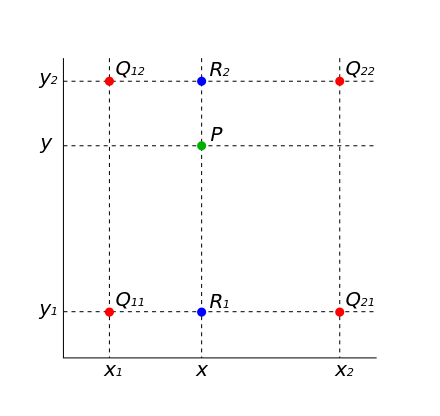
\includegraphics[width=.2\textwidth]{Images/BilinearInterpolation.png}
\end{figure}
\item Polynomial interpolation: Generalisation of linear interpolation with highest degree polynomial equation. For a n-data point problem, there is exaclty one polynomial of degree at most $n-1$ which fit perfectly the data point. Pb: oscillatory effect and computational intensive.
\item Spline Interpolation: is a piecewise polynomial. 
\end{itemize}
Exemple of nearest neighbor (left), linear (center) and polynomial (right) . Note that spline look exacltly similar than polynomial in this exemple.
\begin{figure}[H]
	\centering
	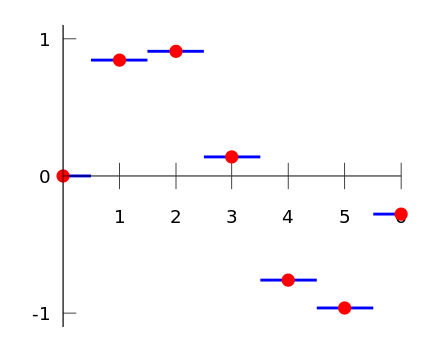
\includegraphics[width=.15\textwidth]{Images/440px-Piecewise_constant.png}
	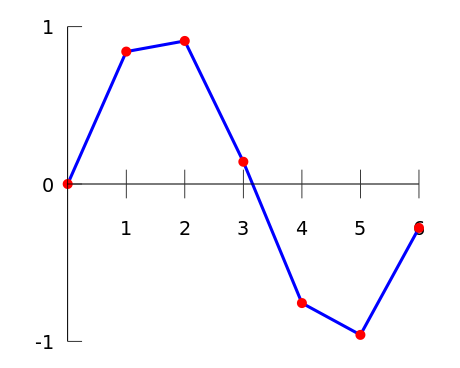
\includegraphics[width=.15\textwidth]{Images/460px-Interpolation_example_linear.png}
	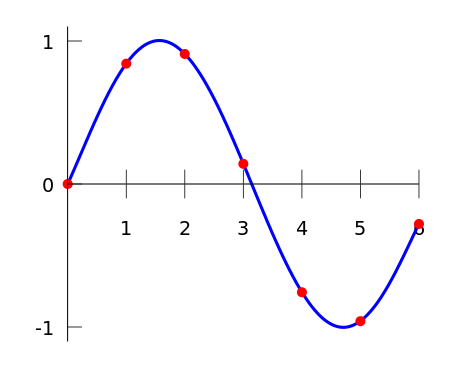
\includegraphics[width=.15\textwidth]{Images/460px-Interpolation_example_polynomial.png}
\end{figure}

\subsection{History and Developement}
The theoretical basis for the method was developed by the French mathematician Georges Matheron based on the Master's thesis of Danie G. Krige (1951), the pioneering plotter of distance-weighted average gold grades at the Witwatersrand reef complex in South Africa. Krige sought to estimate the most likely distribution of gold based on samples from a few boreholes.


\subsection{Variogramm}
The variogram $2\gamma(\boldsymbol{u_1},\boldsymbol{u_2})$ is a function describing the degree of spatial dependence of a spatial random field $Z(\boldsymbol{u})$.
\begin{align*}
2\gamma(\boldsymbol{u_1},\boldsymbol{u_2}) 	&=\text{var} \left(Z(\boldsymbol{u_1}) - Z(\boldsymbol{u_2})\right) \\
  											&= E\left[((Z(\boldsymbol{u_1})-m(\boldsymbol{u_1}))-(Z(\boldsymbol{u_2}) - m(\boldsymbol{u_1})))^2\right]
\end{align*}
For first order stationary $m(\boldsymbol{u_1})=m(\boldsymbol{u_2})$ and with $\boldsymbol{h}=\boldsymbol{u_2}-\boldsymbol{u_1}$
$$2\gamma(\boldsymbol{h}) =E\left[(Z(\boldsymbol{u_0})-Z(\boldsymbol{u_0+h} ))^2\right]$$

\begin{itemize}
	\item nugget $n$: The height of the jump of the semi-variogram at the discontinuity at the origin.
	\item sill $s$: Limit of the variogram tending to infinity lag distances.
	\item range $r$: The distance in which the difference of the variogram from the sill becomes negligible.
\end{itemize}

\begin{tabular}{lcc}
Name			& $\gamma(h)$  & $C(L)$  \\
\hline
Exponential 	& $C_0 \left[1-\exp\left(\frac{-3L}{r}\right)\right]$ 	& $C_0 \exp\left(\frac{-3L}{r}\right)$\\
Spherical		& $C_0 \left[\frac{3L}{2r}-\frac{L^3}{2r^3}\right]$		& $C_0 \left[1-\frac{3L}{2r}+\frac{L^3}{2r^3}\right]$ \\
Gaussian 		& $C_0 \left[1-\exp\left(\frac{-3L^2}{r^2}\right)\right]$& $C_0 \exp\left(\frac{-3L^2}{r^2}\right)$\\ 
\multicolumn{3}{c}{no-sill (Fractional Gaussian Noise or Brownian Motion)}\\
Logarithmic 	& $C_0 \log L$&\\
Sin		 		& $C_0\left[1-\frac{\sin(rL)}{L}\right]$ 				& $C_0\frac{\sin(rL)}{L}$\\
Cos		 		& $C_0\left[1-\cos(rL)\right]$ 							& $C_0\cos(rL)$\\
\end{tabular}


%%%%%%%%%%%%%%%%%%%%%%%%%%%%%
\section{Kriging Basic Description}

\subsection{General Definition}
All kriging version are elaborations of the regression of the following linear combination:
\begin{equation} \label{eq:krig1}
	Z^* (\boldsymbol{u_0}) -m(\boldsymbol{u_0}) =  \sum_{\alpha=1}^{n(\boldsymbol{u_0})} \lambda_\alpha \left[  Z(\boldsymbol{u_\alpha}) - m(\boldsymbol{u_\alpha})\right]
\end{equation}
	
This express the unknown value $Z^*$ at the location $\boldsymbol{u}$ as a linear combination of value $Z$ at the neighbouring point $\boldsymbol{u_\alpha} \in W(\boldsymbol{u_0})$. $\lambda_\alpha$ is the relative importance of each point. And $m(\boldsymbol{u}) =\operatorname{E}[Z(\boldsymbol{u})]$ is the location-dependant expected value.

As the point $\boldsymbol{u_0}$ and $\boldsymbol{u_\alpha}$ are close, it is assumed that their local means are the same : $m_0 = m(\boldsymbol{u_\alpha}) = m(\boldsymbol{u_0})$. The renaming convention $\tilde{Z^*_0} =  Z^* (\boldsymbol{u_0})-m_0$ and $ \tilde{Z_\alpha} =Z(\boldsymbol{u_\alpha}) - m_0$ lead to two variation of Equation~\ref{eq:krig1}
\begin{equation} \label{eq:krig2}
	 Z_0^* =  \sum_{\alpha=1}^{n_0}\lambda_\alpha Z_\alpha + \left( 1- \sum_{\alpha=1}^{n_0} \lambda_\alpha\right) m_0
\end{equation}
\begin{equation} \label{eq:krig3}
	\tilde{Z^*_0} = \sum_{\alpha=1}^n \lambda_\alpha \tilde{Z_\alpha} 
\end{equation}
In this equation, the three unknowns are $\lambda_\alpha$, $m_0$ and $\tilde{Z^*_0}$


\subsection{MVUE}
The minimum-variance unbiased estimator (MVUE) is the estimator which is accurate as well as precise.
\begin{itemize}
	\item Unbiasedness: $\operatorname{B}( \theta^*) = \operatorname{E}[\theta^*]-\theta= \operatorname{E}[\theta^*-\theta]=0$. The bias is the difference between this estimator's($\theta^*$) expected value and the true value of the parameter ($\theta$) being estimated. 
	\begin{align*}
		\operatorname{B}(Z^*_0)	&= \operatorname{E}[Z_0] - \operatorname{E}[Z^*_0]\\
		  						&= \sum_{\alpha=1}^{n_0} \lambda_\alpha \operatorname{E}\left[Z_\alpha \right] + \left( 1- \sum_{\alpha=1}^{n_0} \lambda_\alpha\right) m_0 - \operatorname{E}[Z^*_0]\\
		 						&= \sum_{\alpha=1}^{n_0} \lambda_\alpha m_0 +m_0 - \sum_{\alpha=1}^{n_0} \lambda_\alpha m_0  -m_0\\
		 						&= 0
	\end{align*}
	Bias is always achieved for all method.
	\item Lowest variance: ${\sigma^2_E}^*=\operatorname{var}\{\theta^*-\theta\}$. Minimizing this variance try to not only be accurate but also precise. We can rewritten the equation using notation of equation~\ref{eq:krig2}:
	\begin{align} \label{eq:variance}
		{\sigma^2_E}^* 	&= \operatorname{var} \left\{ Z_0-Z^*_0 \right\} \nonumber\\
						&= \operatorname{var} \left\{ (Z_0-m_0) - (Z^*_0-m_0) \right\} \nonumber\\
						&= \operatorname{var} \left\{ \tilde{Z_0}-\tilde{Z^*_0} \right\} \nonumber \\
						&= \operatorname{var} \left\{ \tilde{Z_0}-\tilde{Z^*_0} \right\} \nonumber \\
						&= \operatorname{var}\left\{\tilde{Z_0}\right\}  +  \operatorname{var}\left\{\sum_{\alpha=1}^n \lambda_\alpha \tilde{Z_\alpha}\right\} -  2 \operatorname{C}\left\{\tilde{Z_0},\sum_{\alpha=1}^n \lambda_\alpha \tilde{Z_\alpha}\right\} \nonumber\\
						&= \operatorname{var}\left\{\tilde{Z_0}\right\}    + \sum_{\alpha=1}^n \sum_{\beta=1}^n \lambda_\alpha \lambda_\beta \operatorname{C}\left\{\tilde{Z_\alpha},\tilde{Z_\beta}\right\} \nonumber \\
						& \quad \quad \quad \quad \quad \quad  \quad \quad  \quad - 2 \sum_{\alpha=1}^n \lambda_\alpha \operatorname{C}\left\{\tilde{Z_0}, \tilde{Z_\alpha}\right\}
	\end{align}
	using,
	\begin{itemize}
		\item $\operatorname{var}\left\{ X -Y \right\} = \operatorname{var}\left\{ X \right\} + \operatorname{var}\left\{ Y \right\} - \operatorname{C}\left\{ X,Y \right\}$
		\item $\operatorname{var}\left\{ \sum_{i=1}^{n} a_iX_i\right\} = \sum_{i=1}^{n} \sum_{j=1}^{n} a_i a_j \operatorname{C}[X_i,X_j]$
	\end{itemize}
\end{itemize}

%%%%%%%%%%%%%%%%%%%%%%%%%%%%%
\section{Method}
\subsection{Simple Kriging}
Simple Kriging (SP) assume location-independent mean $m_0 =m$ (first order stationarity) which mean that the mean is the same throughout the study area (an not only around the simulated point). The mean can be estimated with all known point ($m=\sum Z_i$) and $\lambda_\alpha$ is the only unknown left. This can be find by minimizing ${\sigma^2_E}^*$ which is found when his derivative is equal to 0 for each $\lambda_\alpha$ :
\begin{equation}
	\frac{\partial {\sigma^2_E}^*}{\partial \lambda_\alpha } = 0=2 \sum_{\beta=1}^n \lambda_\beta \operatorname{C}\left\{\tilde{Z_\alpha},\tilde{Z_\beta}\right\}
	-2 \operatorname{C}\left\{\tilde{Z_0}, \tilde{Z_\alpha}\right\}
\end{equation}
Which can be rewritten:
\begin{equation} \label{eq:minimvar}
	\sum_{\beta=1}^n \lambda_\beta \operatorname{C}\left\{\tilde{Z_\alpha},\tilde{Z_\beta}\right\} = \operatorname{C}\left\{\tilde{Z_0}, \tilde{Z_\alpha}\right\}  \quad \text{for } \alpha=1,...,n
\end{equation}
A this point, we want to come back to normal notation ($Z$ instead of $\tilde{Z}$). 
\begin{align*}
		\operatorname{C}\left\{ \tilde{X},\tilde{Y}\right\} 	&= \operatorname{E}[ (X-m_0)(Y-m_0) ] - \operatorname{E}[(X-m_0)] \operatorname{E}[(Y-m_0)]\\
															&= \operatorname{E}[ XY -m_0X -m_0Y+m_0^2]  \\
															&\quad \quad \quad \quad \quad \quad \quad \quad \quad - ( \operatorname{E}[X] - m_0 )( \operatorname{E}[Y] - m_0 )\\
															&= \operatorname{E}[XY] - m_0\operatorname{E}[X] -m_0 \operatorname{E}[Y] + m_0^2 \\
															&\quad \quad \quad \quad -  \operatorname{E}[X] \operatorname{E}[Y] +m_0 \operatorname{E}[X] + m_0 \operatorname{E}[Y] -m_0^2\\
															&= \operatorname{E}[XY] -  \operatorname{E}[X] \operatorname{E}[Y]\\
															&= \operatorname{C}\left\{ X,Y \right\}
\end{align*}
This can be rewrite as a matrix notation and can be identify as an linear system:
\[
		\begin{bmatrix}
       		\operatorname{C}\left\{Z_1,Z_1\right\} 	& \cdots & \operatorname{C}\left\{Z_1,Z_n\right\}   \\
       		\vdots 												& & \vdots 												\\
       		\operatorname{C}\left\{Z_1,Z_n\right\}  & \cdots & \operatorname{C}\left\{Z_n,Z_n\right\}
     	\end{bmatrix}
     	\begin{pmatrix}
       		\lambda_1 	\\
       		\vdots 		\\
       		\lambda_n  
     	\end{pmatrix}
     	=
     	\begin{bmatrix}
       		\operatorname{C}\left\{Z_1,Z_0\right\} \\
       		\vdots 												\\
       		\operatorname{C}\left\{Z_n,Z_0\right\} 
     	\end{bmatrix}
\]   
The $\lambda$ can be found with $\boldsymbol{\Lambda} = \boldsymbol{C_{\alpha,\beta}^{-1}} \boldsymbol{C_{\alpha,0}} $, equations~\ref{eq:krig1} or \ref{eq:krig3} is used to find the estimator $Z_0^*$.

We can put back the minimized solution (equation~\ref{eq:minimvar}) into the variance equation~\ref{eq:variance} :
\begin{equation}
	{\sigma^2_E}^*  = \operatorname{var}\left\{Z_0\right\} - \sum_{\alpha=1}^n \lambda_\alpha \operatorname{C}\left\{Z_0, Z_\alpha\right\}
\end{equation}
The error variance in the estimation is equal to the variance of the data $\operatorname{var}\left\{Z_0\right\}$ reduced by the information brought by  point in the neighbourhood of $\boldsymbol{u_0}$. Note that we used the covariance, but variogram could be interchangeably used 



\subsection{Ordinary Kriging}
Ordinary Kriging doesn't assume first-order stationary ($m_0$ is unknown). In this case, in order to satisfy equation~\ref{eq:krig3}, it is useful to remove the second part of the equation by setting 
\begin{equation} \label{eq:cond}
	\sum_{\alpha=1}^{n_0} \lambda_\alpha=1
\end{equation}
This times, minimizing the variance ${\sigma^2_E}^*$ is more trick as it is subject to equation~\ref{eq:cond}. Solution is find using the method of the Lagrangian multiplier. It is a strategy for finding the local minima $\boldsymbol{u_0}$ of a function $f(\boldsymbol{u})$ subject to equality constraints $g(\boldsymbol{u})=0$. The Lagrangian function is define as: $ F(\boldsymbol{u},2\mu) = f(\boldsymbol{u}) + 2\mu g(\boldsymbol{u})$. This idea behind this method is that if $\boldsymbol{u_0}$ is a minimum point, then there is a point $\mu_0$ such that $(\boldsymbol{u_0}, \mu_0)$ is a stationary point for the lagrangian function. Stationary point are points where all partial derivatives of F are zero $ \nabla_{\boldsymbol{u},\mu} F(\boldsymbol{u_0}, \mu_0)=0 $

In our case the Lagrangian function is:
\begin{equation}
	F(\lambda_\alpha, 2\mu) = {\sigma^2_E}^* + 2\mu \left( \sum_{\alpha=1}^{n_0} \lambda_\alpha - 1\right)
\end{equation}
Leading up to finding the stationary point
\begin{equation} \label{eq:stationnary_pt}
	\left[
	\begin{array}{rl}
		\frac{\partial F}{\partial \lambda_\alpha } &=  \sum_{\beta=1}^n \lambda_\beta \operatorname{C}\left\{Z_\alpha,Z_\beta\right\}
		- \operatorname{C}\left\{Z_0, Z_\alpha \right\}  + \mu \\
		\frac{\partial F}{\partial \mu } &= \sum_{\alpha=1}^{n_0} \lambda_\alpha - 1\\
	\end{array}
	\right]=0
\end{equation}

The procedure is similar to simple kriging but with a new constraint in our system.
\[
		\begin{bmatrix}
       		\operatorname{C}\left\{Z_1,Z_1\right\} 	& \cdots 	& \operatorname{C}\left\{Z_1,Z_n\right\} & 1  		\\
       		\vdots 									& 			& 										& \vdots 	\\
       		\operatorname{C}\left\{Z_1,Z_n\right\}  	& \cdots 	& \operatorname{C}\left\{Z_n,Z_n\right\}	& 1			\\
       		1										& \cdots	 	& 1										& 0
     	\end{bmatrix}
     	\begin{pmatrix}
       		\lambda_1 	\\
       		\vdots 		\\
       		\lambda_n	\\
       		\mu  
     	\end{pmatrix}
     	=
     	\begin{bmatrix}
       		\operatorname{C}\left\{Z_1,Z_0\right\} 	\\
       		\vdots 									\\
       		\operatorname{C}\left\{Z_n,Z_0\right\} 	\\
       		1
     	\end{bmatrix}
\] 

Once the $\lambda$ have been found, equation~\ref{eq:krig3} can be simplified and help us compute the value at the unsample location.
\begin{equation}
	Z_0^* =  \sum_{\alpha=1}^{n_0}\lambda_\alpha Z_\alpha
\end{equation}

In a similar matter, variance of the computed value can be found with
\begin{equation}
	{\sigma^2_E}^*  = \operatorname{var}\left\{Z_0\right\} - \sum_{\alpha=1}^n \lambda_\alpha \operatorname{C}\left\{Z_0, Z_\alpha\right\} -\mu
\end{equation}




\subsection{Kriging with a Trend}
The assumption made in the general description that the mean is constant in the search neighbour $m(\boldsymbol{u_0}) = m(\boldsymbol{u_\alpha}) ,\alpha \in W(\boldsymbol{u_0})$ might not hold in the presence of a trend. In the Universal Kriging (with a trend), the local mean in a search neighboor is modelled with a smoothly varying function:
\[ m(\boldsymbol{u_\alpha})=\sum_{k=0}^K{a_k f_k(\boldsymbol{u_\alpha})}\]
Where $f_k$ are known function while the coefficient $a_k$ are unknown. Note that if k=0, we end up with Ordinary Kriging. Equation~\ref{eq:krig3} became:
\begin{equation}
	Z_0^* =  \sum_{\alpha=1}^{n_0}\lambda_\alpha Z_\alpha + \left( f_{k,0} - \sum_{\alpha=1}^{n_0} \lambda_\alpha f_{k,\alpha} \right) \sum{k=0}^K a_k
\end{equation}
We follow the same procedure as Ordinary kriging and find a similar equation to equation~\ref{eq:stationnary_pt}
\begin{equation} 
	\left\{
	\begin{array}{ll}
		\operatorname{C}\left\{Z_0, Z_\alpha \right\} &=  \sum_{\beta=1}^n \lambda_\beta \operatorname{C}\left\{Z_\alpha,Z_\beta\right\}
		  + \sum_{k=0}^K \mu_k f_{k,\alpha}  \\&\hfill \text{for } \alpha= 1,...,n_0\\
		f_{k,0} &= \sum_{\alpha=1}^{n_0} \lambda_\alpha f_{k,\alpha} \\& \hfill \text{for } k= 0,...,K\\
	\end{array}
	\right.
\end{equation}
\begin{equation}
		\begin{bmatrix}
       		[\operatorname{C}\left\{Z_\alpha,Z_\beta\right\}]	& [f_{k,\alpha}]^T	\\
       		[f_{k,\beta}]							& [0	]						\\
     	\end{bmatrix} 
     	\begin{pmatrix}
       		[\lambda_\beta]^T 	\\
       		[\mu_k]^T 		\\
     	\end{pmatrix}
     	=
     	\begin{bmatrix}
       		[\operatorname{C}\left\{Z_\alpha,Z_0\right\}]^T 	\\
       		[f_{k,0}]^T 					\\
     	\end{bmatrix}
\end{equation}
Once the $\lambda_\beta$ and $\mu_k$ are found, kriging estimate and variance can be computed.



\subsection{Block Kriging} 
\emph{Block Estimation} is used when the estimated location is not a point but has an area. In this case, the estimator is assumed to be the arithemic average of all point inside the volume ($\boldsymbol{u_{0,i}}$):
\[ Z_V^*( \boldsymbol{u_{0}}) = \frac{1}{N} \sum_{i=0}^N Z^*(\boldsymbol{u_{0,i}})\]
This is a arithmeric average and transformation might be necessary. The procedure is similar to ordinary (or simple) kriging except that the covariance between the known point and unknown volume is computed by averaging the covariance between known point and point inside the volume
\[ C\{Z_{\alpha},Z_{V,0}\}  = \frac{1}{N} \sum_{i=0}^N  C\{Z_{\alpha}, Z_{0,i}\} \]
\begin{equation}
		\begin{bmatrix}
       		[\operatorname{C}\left\{Z_\alpha,Z_\beta\right\}]	& [1]^T	\\
       		[1]							& [0	]						\\
     	\end{bmatrix} 
     	\begin{pmatrix}
       		[\lambda_\beta]^T 	\\
       		[\mu] 		\\
     	\end{pmatrix}
     	=
     	\begin{bmatrix}
       		[\operatorname{C}\left\{Z_\alpha,Z_{V,0}\right\}]^T 	\\
       		[1]					\\
     	\end{bmatrix}
\end{equation}


\subsection{Dual Kriging}
\emph{Dual Kriging} is just a way of presenting kriging where the estimate is express as a linear combination of covariance instead of values. Solution for $\lambda$  ($\boldsymbol{\Lambda} = \boldsymbol{C_{\alpha,\beta}^{-1}} \boldsymbol{C_{\alpha,0}} $) can be incorporated in the general definition of kringing (equation~\ref{eq:krig1}) and lead up to:
\begin{equation} \label{eq:dualkrig}
		Z^* (\boldsymbol{u_0}) -m(\boldsymbol{u_0}) =  \sum_{\alpha=1}^{n(\boldsymbol{u_0})} d_\alpha C\{Z(\boldsymbol{u_\alpha}),Z(\boldsymbol{u_0})  \}
\end{equation}

The weight $d_\alpha$ are obtain by identification of data
\begin{equation}
		\begin{bmatrix}
       		[\operatorname{C}\left\{Z_\alpha,Z_\beta\right\}]		\\
       		[1]													\\
     	\end{bmatrix} 
       	[d_\beta]^T 	\\
     	=
     	\begin{bmatrix}
       		[Z_\alpha]^T - m_0 	\\
       		[0] 					\\
     	\end{bmatrix}
\end{equation}
With dual kriging we are not minimizing an error variance but "calibrate" the weight on the known values. What's really interesting here is that the weight $d_\alpha$ are only depending on $\boldsymbol{u_\alpha}$ and $\boldsymbol{u_\beta}$ but not on $\boldsymbol{u_0}$. This made possible to compute the weight once and use them for several point.

\subsection{Filtering}
One exemple of filtering is with a nugget effect: we don't want the direct neighbouring point ($Z(\boldsymbol{u_{min}})$ with $\| \boldsymbol{u_{min}}-\boldsymbol{u_0}\|< d_{min}$) to influence the estimated value. Equation~\ref{eq:dualkrig} helps us to see how filtering can be apply to krigging by simply putting covariance at certain distance equal to zero. 


\subsection{Non-linear Kriging}
 \emph{Log-Normal Kriging} is a non-linear krigging procedure which (1) reduces the variability of sample point and (2) transform log-normal distributed variables in normale distribution. The back-transforme depend on error variance. (not very used)
\emph{Multi-gaussian} convert with a normal z-score the data. 

\subsection{Indicator Kriging} final result represent the uncertain distribution at unsampled location (instead of single value) and has not simple back transform which therefore require a conditional simulation technique. Indicator variable express the confidence in the sample values. It therefore allows incomplete or soft information (value less than 1). There are not distribution assumed in the data.
\[I(u_j,x_t) = \left\{
	\begin{array}{l}
		1 \text{, if }X(u_j)<x_t\\
		0 \text{, if }X(u_j)>x_t
	\end{array}
\right.\]	


%%%%%%%%%%%%%%%%%%%%%%%%%%%%%
\section{Multivariate Kriging}
\subsection{Cokriging}
\emph{Cokriging} is used to estimate one variable (primary $Z$) value knowing other sampled variables (covariables $Y$). It use the assumption that the variables are spatially related with a linear relationship. The relationship must be strong: (1) high correlation, (2) physical link and (3) good history matching. This procedure is very computer expensive and numerical unstable.


The procedure is similar, this time the estimate is a weighted linear combination of the surrounding value of the primary and those of the secondary variable. In order to find the weight, in addition to the covariance structure of the primary variable ($C{Z_\alpha,Z_\alpha}$), we also need the one of the secondary variable ($C{Z_\alpha,Y_\beta}$) and the cross-covariance of both ($C{Y_\alpha,Y_\beta}$).
\begin{equation} \label{eq:cokrig}
	\tilde{Z^*_0} = \sum_{\alpha^Z=1}^n \lambda_{\alpha^Z}^Z \tilde{Z_{\alpha^Z}} + \sum_{\alpha^Y=1}^m \lambda_{\alpha^Y}^Y \tilde{Y_{\alpha^Y}} 
\end{equation}

In ordinary cokriging, we need $m_{Z,0} -\sum_\alpha^Z \lambda_{\alpha^Z}^Z m_{Z,0} - \sum_\alpha^Y \lambda_{\alpha^Y}^Y m_{Y,0} = 0$, which is achives for both $\sum_\alpha \lambda_\alpha = 1$ (as usual) and $\sum_\beta \lambda_\beta = 0$. This additional constraint can be put in the matrix format :

\[
		\begin{bmatrix}
       		\operatorname{C}\left\{Z,Z\right\} 	& \operatorname{C}\left\{Z,Y\right\} 	& [1]_{n\times 1}	& [0]_{n\times 1} 	\\
       		\operatorname{C}\left\{Y,Z\right\}  	& \operatorname{C}\left\{Y,Y\right\}		& [1]_{n\times 1}	& [0]_{n\times 1} 	\\
       		[1]_{1\times n}						& [0]_{1\times n}						& 0		& 0	\\
       		[0]_{1\times n}						& [1]_{1\times n}						& 0		& 0	\\
     	\end{bmatrix}
     	\begin{pmatrix}
       		\lambda_{Z} 	\\
       		\lambda_{Y}	\\
       		\mu_{Z} \\ 
       		\mu_{Y} \\
     	\end{pmatrix}
     	=
     	\begin{bmatrix}
       		\operatorname{C}\{{Z_0,Z}\} 	\\
       		\operatorname{C}\{{Z_0,Y}\}	\\
       		1 	\\
       		0\\
     	\end{bmatrix}
\] 


\subsection{Kriging with external Drift}

\subsection{Collocated cokriging}

\subsection{Cosimulation}

\subsection{...}



%%%%%%%%%%%%%%%%%%%%%%%%%%%%%
\section{Search Strategie}
Search strategie  are used in computing covariance matrices. Three reasons encourages algorithm to only a limited number of neraby conditioning data : 
\begin{enumerate}
	\item CPU time to solve a kriging system is $\mathcal{O}({n^3})$ and memory storage is $\mathcal{O}({n^2})$,
	\item Knowlegde of covariance for very distence over half or third of domain is poorly known 
	\item  local search allow local rescaling of the mean for ordinary kriging.
\end{enumerate} 
 
Three technique will be explained:
\begin{itemize}
\item The simplest implementation is to check for all available point and retaining only the one inside the ellipsoid (Exhaustive search).
The previous work was sorting the point and selecting the n-closest \citep{Ruggeri2013}
\item Composite sampling presented in \citep{isaaks1989introduction} selects the n-closest points and then split the remaining point into quadrant (or octant). When building the covariance matrix, points on each quadrant are being treated as block points. This results in a similar weight for all points inside the same quadrant.
\item The super Block Search \citep{deutsch1998gslib,Lyster2008} consist of creating a coarse grid network surimposing the data and associated each data point to its corresponding block. When searching the neighbourhood, distance is computed on super blocks center, retaining those blocks following inside the ellipse, and all data points contained in the selected blocks are used for kriging. This method is particularly useful for scatter data with an unchanging number of point. The number (and size) of the blocks is a critical parameter to avoid boundary artefact.
\item Spiral Search \citep{deutsch1998gslib} is very efficient for regular gridded data as it looks sequentially at all grid nodes starting by the closer one and going further away. It can stop whenever a certain number of point is reached.
\item Quadrant Search is especially interesting for clustered data as it splits the search window in 4 (or 8 in 3D) zones and can limit the number of points in each quandrant (or octant) separately. This force an equal directional sampling.
\item For gridded sequential simulation with scattered conditioning hard data, a two-part search combining both super block search for hard data and spiral search for previously simulated point is suggested by \cite{deutsch1998gslib}. One advantages is that hard data can be selected in a different manner than previously simulated point and therefore it is possible to give a special effort to reproduce the hard data effect.
\item Search Tree Structure \citep{Manchuk2004} successively divide the space in quandrant (or octant for 3D) indexing each region. In this way, different area of the space are sub-divided at different level. The nearest search become a simple query on the tree using the index of the region to find the corresponding nearest point. The memory usage is particularly low because each node only store its parent nodes up to the root. This method is useful for unstructured grids.
\end{itemize}

Cross validation of subspace can help to select the search criteria.


\section{Limitation}
\begin{itemize}
	\item 1st order stationary (mean cst) required
	\item Only applicable for Gaussian-related stochastic model
	\item if search long enough : global minima is achieved.
	\item In theory, spacial structure is preserve. But in practise, because each simulation is not perfect (exact mean, variance and covariance) spatial statistical structure is not preserve. This become a serious problem when the number of realisation is higher than the number of grid cells (see \cite{Hu2002})
	\item Preserve only variogram structure (covariance) not multi-point
	\item for linear problems, GDM's optimizations  converge exponentially to the global minimum but not for non linear. 
	\item Something about getting accurate estimate... using a prior constraint \cite{LeRavalec-Dupin2002}
\end{itemize}

\section{To go futher}
\begin{itemize}
\item Cross validation
\item 
\end{itemize}




\bibliographystyle{apalike}
\bibliography{citations}	
	

\end{document}
